\documentclass[addpoints,12pt]{exam}
\usepackage{amsmath,amsthm,amssymb}
\linespread{1.05}
\usepackage{hyperref}
\usepackage[top=0.5in,bottom=1in,left=1in,right=1in]{geometry}
\usepackage[linesnumbered,ruled]{algorithm2e}
\usepackage[dvipsnames]{xcolor}
\usepackage{tikz}
\usepackage[framemethod=TikZ]{mdframed}

\usepackage{graphicx}
\graphicspath{ {./images/} }

\usepackage{tcolorbox}
\tcbuselibrary{theorems}

\newtcbtheorem[number within=section]{theo}{Theorem}%
{colback=green!5,colframe=green!35!black,fonttitle=\bfseries}{th}

\newtcbtheorem[number within=section]{hypothesis}{Hypothesis}%
{colback=red!5,colframe=red!35!black,fonttitle=\bfseries}{th}

\newtcbtheorem[number within=section]{define}{Definition}%
{colback=blue!5,colframe=blue!35!black,fonttitle=\bfseries}{th}


\printanswers
\marksnotpoints

\pointformat{\textcolor{Maroon}{(\thepoints)}}
\qformat{\textcolor{Maroon}{\textbf{Problem~\thequestion}} \hfill \textcolor{Maroon}{\textbf{\totalpoints~\points}}}


\newcommand{\course}{{\large CS6170: \textsc{Randomized} \textsc{Algorithms}}}
\newcommand{\pset}[1]{{\large \textsc{Problem} \textsc{Set} \##1}}
\newcommand{\due}[1]{{\textsc{Due}: #1}}
\newcommand{\name}[1]{\textsc{Name}: \textcolor{Blue}{#1}}
\newcommand{\rno}[1]{\textsc{Roll} \textsc{No}: \textcolor{Blue}{#1}}
\pagestyle{plain}

\DeclareMathOperator{\Var}{Var}
\newcommand{\E}{\mathbb{E}}
\DeclareMathOperator{\Poi}{Poi}


\begin{document}
	
	\hrule height 2pt
	\vspace{2mm}
	{\centering \course \par}
	\vspace{1mm}
	{\centering \pset{4}\par}
	\vspace{1mm}
	\noindent \name{Akash Roy} \\
	\rno{CS22M007}\hfill \due{Oct 24, 23:59}
	\vspace{2mm}
	\hrule height 2pt
	\vspace{2mm}
	
	\begin{questions}
		
		\question Consider the following deterministic paging algorithms.
		\begin{itemize}
			\item Longest-Time First: Whenever there is a cache-miss evict the item that has been in the cache for the longest period of time.
			\item Least Frequently Used: Whenever there is a cache-miss, evict the item that has been requested least often.
		\end{itemize}	
		\begin{parts}
			\part[3] Show that the LTF paging scheme is $k$-competitive where $k$ is the size of the cache.
			\begin{solution}
				For any consecutive requests that involve $\leq k$ distinct elements, longest time first algorithm spends at most $k$ many evicts. Thus making it a conservative paging algorithm.

                \begin{theo}{}{theoem1}
                  \textit{Any conservative paging algorithm is $k$-competitive.}
                \end{theo}

                From theorem 0.1 it is \textbf{enough} to show LTF is a conservative algorithm. For the first sub-sequence of $k$ distinct requests LTF will not evict anyone. For the next $k$ distinct requests see the analysis below:

                Say $X$ is the first of such requests. There can be 2 cases first $X \in$ LTF's cache then there is no miss or $X \in$ LTF's cache or not. If it is not then there will be one miss. For LTF's algorithm there can be atmost $k$ many misses for the next $k$ distinct requests because it's removing the oldest page from the cache. So it must be a conservative paging algorithm.

                \textbf{Proof. of theorem 0.1} For a stretch of $k$ distinct element subsequence conservative algorithm will miss at most $k$ faults via definition. 

                Say OPT added $k$ distinct elements in the cache from the first subsequence. For the first element of the second subsequence $X$ say $X \in$ OPT's cache. Then there is no fault. If $X \notin$ OPT's cache then it'll remove the one that's referenced furthest in future. There is $k$ distinct element in the cache so it'll remove one element that'll not be requested for next $k-1$ many requests. So therefore there is 1 fault.

                $$\text{COST}_{\text{conservative}} \leq k * \text{COST}_{\text{OPT}}$$
			\end{solution}
			\part[3] Show that the competitive ratio for LFU is unbounded.
			\begin{solution}
				LFU is not a conservative algorithm but that does not guarantee the fact that it is not $k$-competitive via theorem 0.1. Consider the following sequence of operations with cache size $k = 4$,

                $$\{1,2,3,1,2,3,4,5,4,5,4,5,4,5 \dots\}$$
                For the first $6$ operations the keys 1, 2, 3 will have frequencies set to $2$ then for the $7^{th}$ request frequency of $4$ will be set to 1. So for incoming request $5$, $4$ will be removed from the cache. Now for any subsequence of size $l > 2$ with 2 distinct element in the request line there is more than 2 faults. So LFU is not a conservative algorithm.

                For requests going to the infinity the number of faults will increase and continue to increase. OPT algorithm will not have that problem because it'll see that 1, 2, 3 is not referenced again so it'll remove those to accommodate request 5, so the cost of OPT will be 2. So then LFU will have unbounded competitive ratio depending upon the size of the requests not the size of the cache.
			\end{solution}
		\end{parts}
	
		\question An \emph{edge coloring} of a graph is an assignment of colors to the edges of a graph such that no two edge that share a vertex are assigned the same color. Let us look at the online version of edge coloring where the number of vertices in the graph are fixed, and the edges arrive in an online fashion. We will assume that the degree of every vertex in the graph is at most $\Delta$.
		
		\begin{parts}
			\part[3] Show that there exists an online algorithm that can edge color the graph with at most $2\Delta - 1$ colors.
			
			The best that an online algorithm can be do is $\Delta+1$, and follows from Vizing's theorem in graph theory.
			\begin{solution}
				Discussed with Krishna.\\
                Greedy edge coloring will work, we choose a used color for an edge if it is not shared with already colored one.
                Say an edge $e \in G.E$. Different colors to be used is at most $\mathrm{deg}(u) + \mathrm{deg}(v) - 1 \leq 2\Delta - 1$
			\end{solution}
	
			\part[5] Show that there is no deterministic algorithm that uses fewer than $2\Delta - 1$ colors in the worst case.
			
			To that end, consider a graph consisting of disjoint stars with $\Delta$ vertices, and edges connecting the center vertex of each of the stars to another fixed vertex. Show that for any deterministic algorithm, there is an adversarial order that can force $2\Delta - 1$ colors.
			\begin{solution}
				Type your solution here.
			\end{solution}
			
		\end{parts}
	
		\question[5] When studying the $2$-SAT algorithm, we considered a random walk on a graph $G$ on $n$ vertices. Consider the following modified random walk on that graph. At vertex $v_0$, with probability $1/2$, you remain in $v_0$ and with probability $1/2$ you move to $v_1$. The remaining transition probabilities all remain the same. Compute the expression for the expected time to reach vertex $v_n$ from $v_i$ for such a random walk.
		\begin{solution}
			From the question expected hitting time for all the states are the following [as done in the class]
            \begin{align*}
                h_0 &= \frac{1}{2} h_0 + \frac{1}{2} h_1 + 1\\
                h_1 &= \frac{1}{2} h_0 + \frac{1}{2} h_2 + 1\\
                h_2 &= \frac{1}{2} h_1 + \frac{1}{2} h_3 + 1\\
                \vdots\\
                h_{n-1} &= \frac{1}{2} h_{n-2} + \frac{1}{2} h_n + 1\\
                h_n &= 0
            \end{align*}

            We can expand the equation like the following: 
            \begin{align*}
                h_0 &= \frac{1}{2} h_0 + \frac{1}{2} h_1 + 1\\
                \frac{1}{2} h_0 &= \frac{1}{2} h_1 + 1\\
                h_0 &= h_1 + 2\\
            \end{align*}

            Similarly from last equation we can write for $h_1$
            \begin{align*}
                h_1 &= \frac{1}{2} \left[h_1 + 2\right] + \frac{1}{2} h_2 + 1\\
                \frac{1}{2} h_1 &= 1 + 1 + \frac{1}{2} h_2\\
                h_1 &= 4 + h_2\\
            \end{align*}

            Similarly $h_3$ becomes $h_4 + 8$ and so on. For any general $i$ $h_i$ is $h_{i+1} + 2i + 2$

            Solving this recurrence $h_i = h_{i+1} + 2i + 2$ gives us the expected hitting time for this modified markov chain.
            
            \textbf{Recurrence relation solution} for any $i \in \{1 \to n-1\}$
            \begin{align*}
                h_i &= h_{i+1} + 2(i+1)\\
                &= h_{i+2} + 2(i+2) + 2(i+1)\\
                &= h_{i+k} + 2(i+k) + \dots + 2(i+1)\\
            \end{align*}

            \textbf{SEE NEXT PAGE}
		\end{solution}

        \begin{solution}
            At $i+k = n$ the relation becomes,
            \begin{align*}
                h_i &= h_{i+k} + 2(i+k) + \dots + 2(i+1)\\
                &= h_n + 2n + 2(n-1) + \dots + 2(i+1)\\
                &= 2 \left[\displaystyle\sum_{i=1} ^{n} i - \displaystyle\sum_{i=1} ^{i}\right]\\
                &= n^2 + n - i^2 - i\\
                &= n(n+1) - i(i-1)
            \end{align*}

            Expected time to reach $v_n$ from vertex $v_i$ is $n(n+1) - i(i-1)$.
        \end{solution}
		
		\question A coloring of a graph is an assignment of colors to the vertices in the graph. A graph is said to be $k$-colorable, if there is a coloring of the graph with $k$ colors such that no two adjacent vertices have the same color. Let $G$ be a $3$-colorable graph.
		\begin{parts}
			\part[2] Show that there exists a coloring of the graph with $2$ colors such that no triangle is monochromatic. (A monochromatic triangle is one that has all vertices of the same color.)
			
			\textcolor{red}{Do not use Part (b) to solve this question.}
			\begin{solution}
				Say I color the graph $\mathbb{G}$ which is a $3$-colorable graph using three colors \textbf{\textcolor{red}{red}, black and \textcolor{blue}{blue}}. As the graph is three colorable that means every vertex in triangles present in graph $\mathbb{G}$ in the graph must have 3 different assignment of colors. Now let's change every color \textcolor{red}{red} to \textbf{black}. Now the resultant $\mathbb{G}_{\textcolor{red}{red} \to black}$ is a 2-colored graph and each triangle is not monochromatic.
			\end{solution}
			
			\part[4] Consider the following algorithm for coloring $G$ with two colors so that no triangle is monochromatic. The algorithm begins with an arbitrary $2$-coloring. While there are monochromatic triangles in $G$, the algorithm chooses one such triangle and changes the color of a randomly chosen vertex of the triangle. Derive an upper bound on the expected number of such recoloring steps before the algorithm finds a $2$-coloring with the desired property.
			\begin{solution}
				Say I have a random 2 coloring of a graph. Now It may have some triangles that are monochromatic. I need to find the upper bound on how many recoloring steps all the triangle becomes non-monochromatic and triangles are choosen uniformly at random and vertex to re-color is also choosen u.a.r.

                Say $\mathbb{C}(3)$ is a 3-coloring of the graph $G$ with colors being \textbf{\color{red}{red}, \color{black}{black} and \color{blue}{blue}}. And from the algorithm say $\mathbb{C}(2)$ is any arbitrary 2 coloring of vertices. For $\mathbb{C}(3)$ coloring say $V_{\textbf{red}}, V_{\textbf{black}}, V_{\textbf{blue}}$ are three independent set showing what vertex are colored what?

                For arbitrary 2 coloring $\mathbb{C}(2)$ if all vertex in $V_{\textbf{red}}$ are colored red and all vertices in $V_{\textbf{black}}$ are colored black then we don't need any recoloring in any triangles. So we can make a markov chain with hamming distance being what are the number of vertexes different from $V_{\textbf{black}}$ and $V_{\textbf{red}}$. So I define the distance of Markov chain to be the following
                \begin{align*}
                    \textsc{distance} = \Big\vert \{v \in V_{\textbf{black}} \text{ but color is red}\} \bigcup \{v \in V_{\textbf{red}} \text{ but color is black}\} \Big\vert
                \end{align*}

                In the algorithm one monochromatic triangle is taken at random. It can have 2 possibilities it is either a \textbf{\color{red}{red, red, red}} or a \textbf{black, black, black} triangle.

                If we take the vertex uniformly at random to flip there is 3 possibilities
                \begin{itemize}
                    \item We choose a vertex $V_{blue}$ and flip it. Then the distance remains the same,
                    \item We choose a vertex from $V_{black}$ and it has black color and flip it then we move back one distance, or we choose a vertex from $V_{red}$ and it has red color and flip it then we move back one distance
                    \item We choose a vertex from $V_{black}$ and it has \textcolor{red}{red} color or we choose from $V_{red}$ and it has \textbf{black} color. Then we move distance by one towards the end of the markov chain.
                \end{itemize}
                \bigskip
                
                Hence our Markov chain will be the following:\\
                
                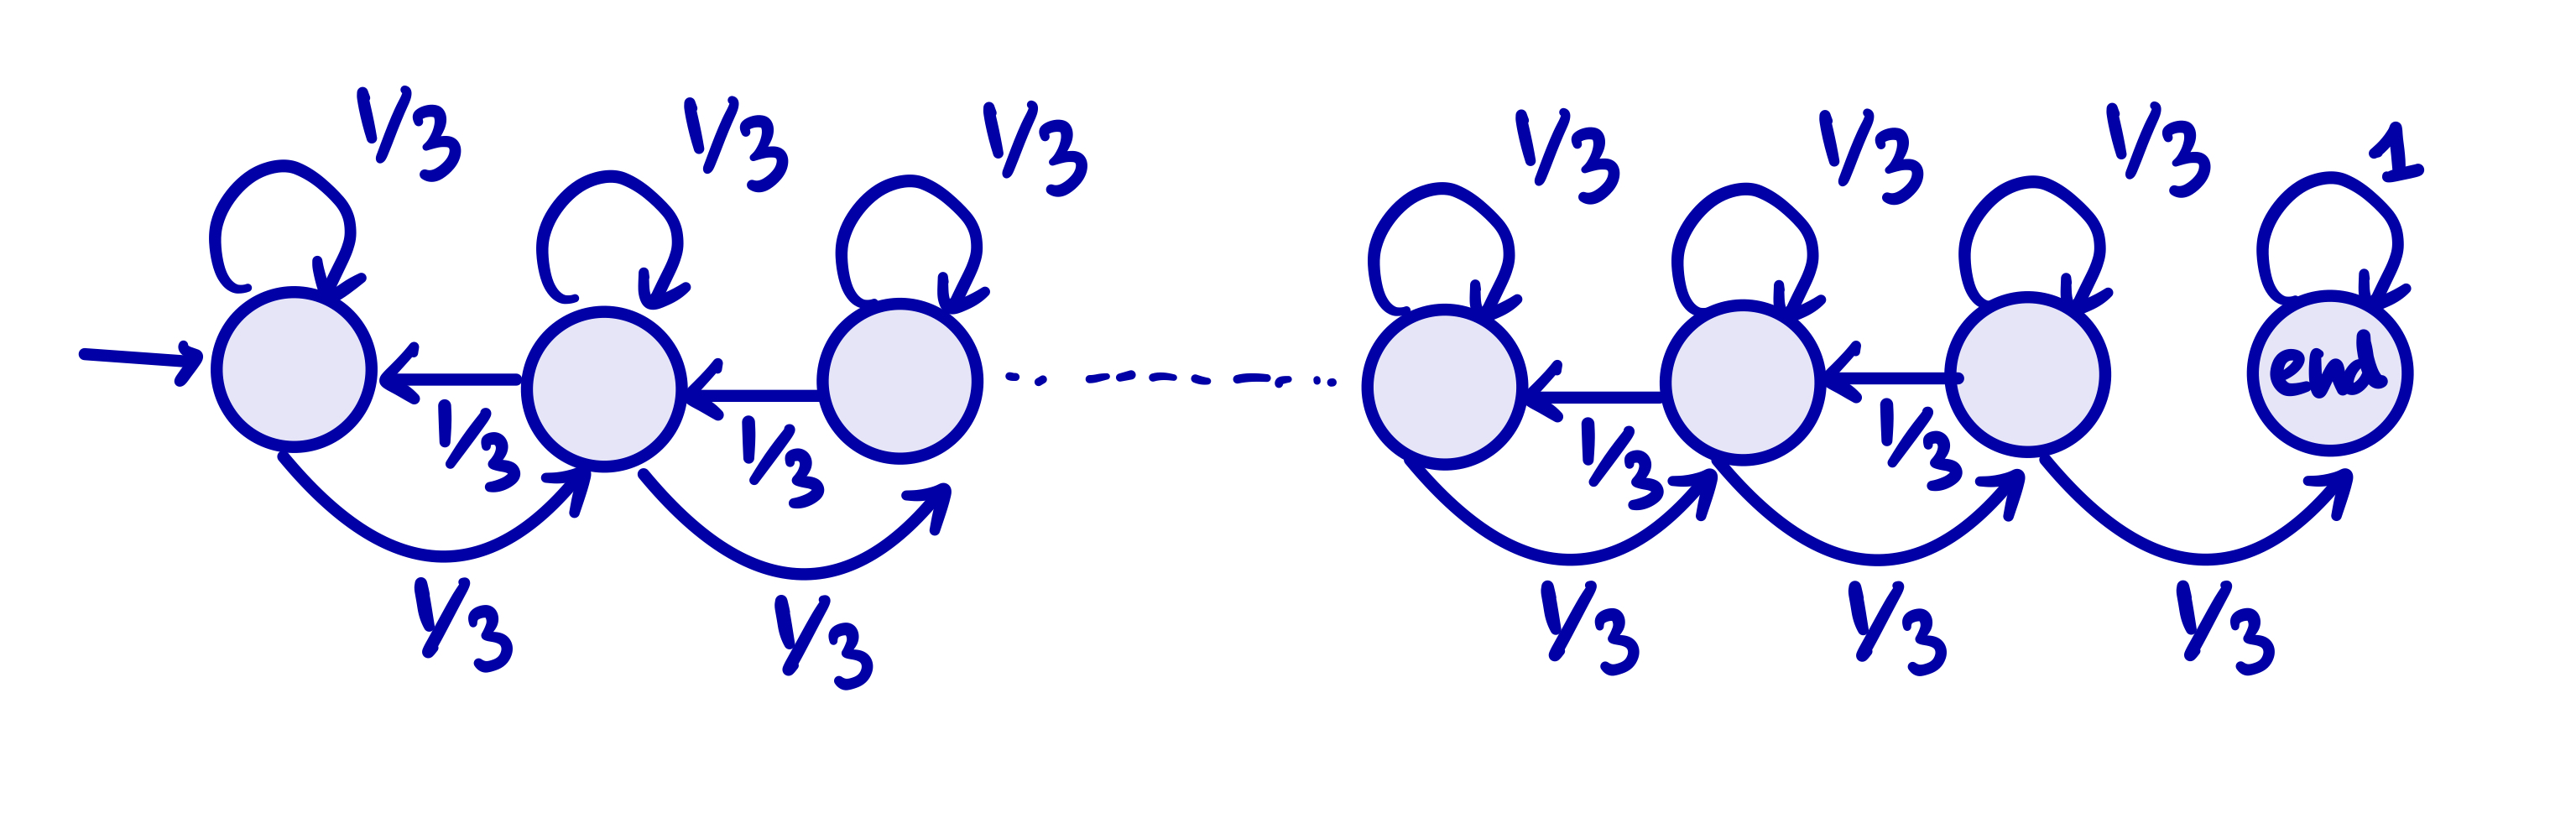
\includegraphics[scale=0.12]{chain}

                For any state $i$ except for the last state \textbf{end}, we can write the following equation with $h_{i \to \text{end}}$ being the time to go from state $i \to \text{end}$
                \begin{align*}
                    h_{i \to \text{end}} &= \frac{1}{3} h_{i \to \text{end}} + \frac{1}{3} h_{i+1 \to \text{end}} + \frac{1}{3} h_{i-1 \to \text{end}}\\
                    \frac{2}{3} h_{i \to \text{end}} &= \frac{1}{3} h_{i+1 \to \text{end}} + \frac{1}{3} h_{i-1 \to \text{end}}\\
                    h_{i \to \text{end}} &= \frac{1}{2} h_{i+1 \to \text{end}} + \frac{1}{2} h_{i-1 \to \text{end}}
                \end{align*}
                Now solving the recurrence with $h_{\text{end} \to \text{end}} = 0$ will give us the time bound for hitting end in the markov chain in $h_{0 \to \text{end}}$ which is $O(n^2)$.
            \end{solution}
		\end{parts}
		
		\question[5] A cat and a mouse each independently take a random walk on a connected, undirected, non-bipartite graph $G$. They start at the same time on different vertices, and each makes one transition at each step. The cat eats the mouse if they are ever at the same vertex at some time step. Let $n$ and $m$ denote the number of vertices and edges in $G$. What is the expected time before the cat eats the mouse?
		
		\begin{solution}
			Our Markov chain will have $n*n = n^2$ new states. The states of the form $i, i \in$ the Markov chain denotes where the cat will eat the mouse. In the new Markov chain each of the state $(i, j)$ is connected to $\mathrm{deg}(i) * \mathrm{deg}(j)$ many nodes. There can be parallel edges in this new Markov chain. Now summing up all the degrees of this new Markov chain will give bound $2E$ where E is the number of edge in the new markov chain (via handshaking lemma).
            
            \begin{align*}
                \displaystyle\sum_{i, j}\mathrm{deg}(i) * \mathrm{deg}(j) &= \displaystyle\sum_{i} \displaystyle\sum_{j}\mathrm{deg}(i) * \mathrm{deg}(j)\\
                &= \displaystyle\sum_{i} \mathrm{deg}(i) * \displaystyle\sum_{j} \mathrm{deg}(i)\\
                &= (2m) * (2m)\\
                &= 4m^2\\
            \end{align*}

            So number of edges in the new Markov chain is $2m^2$. From lemma in class hitting time bound $h_{u,v} \leq 2 \mid E\mid = 4m^2$ if $(u, v)$ are adjacent.

            If there is a path length of size $l$ for each of the node in Markov chain to a node of type $(i, i)$ then the expected time for the mouse to be eaten is $l * O(m^2)$.

            From Mitzenmacher and Upfal exercise 7.22 the bound is $O(m^2 n)$, hence $l$ must be upper bounded by O(n). Hence the upper bound on the time for the cat to eat the mouse is $O(m^2 n)$.
		\end{solution}
	\end{questions}
\end{document}